\section{Local Challenge: Obstacle Avoidance}
\label{sec:ObstacleAvoidance}

\subsection{Idea of the Challenge}

Teams at RoboCup 2019 self-reported working on/having finished improvements of their obstacle avoidance. Replacing simple obstacle avoidance implementations (don't walk forward if you don't see field colour in front of you) should be encouraged by the league. This challenge gives teams to display their improvements in obstacle avoidance. It might aid in lowering the amount of pushing during games.

\subsection{Overview}

Teams are challenged to move a ball into the target goal as fast as possible. Obstacles are placed in-between the ball and target goal. To participate a team needs access to:

\begin{itemize}
	\item a single active NAO robot.
	\item about 75\% of a SPL field.
	\item 3 inactive NAO robots.
	\item SPL robot jerseys.
	\item the ability to stream a video of their field (\cf Section \ref{sec:streaming_setup}).
\end{itemize}

If a team is interested in participating in this challenge, but cannot fulfil all requirements: please send an e-mail to \url{rc-spl-tc@lists.robocup.org}.

\subsection{Judges and Assistants}

The challenge will be judged by a neutral member of another SPL team via video stream. The competing team needs to designate one person as local challenge assistant. The local challenge assistant assists the judge in setting up the challenge, starting and stopping, scoring and moving the ball/obstacles.

\subsection{Setup}

The challenge is attempted on a SPL field (\cf Section \ref{sec:field_dim}) in the local venue of the participating team. One of the goals on the field is designated as the target goal. The other goal is not used as part of the challenge (but remains in place).

A ball is placed in the centre of the centre circle. The challenged robot is placed in front of the centre circle on the opposite side of the of the target goal (equivalent to manual placement of attacking robots during kick-off in SPL games). Between ball and target goal three obstacles are placed.

\begin{itemize}
	% Moving obstacle removed for now to keep accessibility of the challenge high.
	% \item One moving robot as an obstacle. This robot is continuously moving back and forth along an imaginary line oriented along the short axis of the field, facing the direction of travel as it moves. The distance travelled by the robot is approximately the width of the penalty area (see dimension H of section "Field Construction" of the SPL rules).
	\item One stationary robot as an obstacle (\cf Section \ref{sec:stationary_obstacle_robots}), facing down the long dimension of the field, centred on the imaginary line between kick-off point and centre of the target goal.
	\item One stationary robot as an obstacle, facing down the long dimension of the field, offset to the left or right so its outermost shoulder point is one balls radius away from the imaginary line between kick-off point and centre of the target goal. % The stationary robot is standing upright (might be turned off).
	\item Two stationary robots as an obstacle, facing down the long dimension of the field, positioned offset to the sides so dribbling a ball in between them is the fastest route to the target goal. The space in between them is twice the robots' shoulder-to-shoulder width. % Both stationary robots are standing upright.
\end{itemize}

Regarding to the position of the obstacles along the long axis of the field:

\begin{itemize}
	\item One obstacle is placed on the goal box line (see line F in figure \ref{fig:field_dim}).
	\item One obstacle is placed just outside the penalty box, so it does not touch the line (see distance  G).
	\item One obstacle is placed away from the centre line towards the target goal. The distance to the centre line is the radius of the centre circle (half of distance J).
\end{itemize}

\begin{figure}[ht]
	\centering
	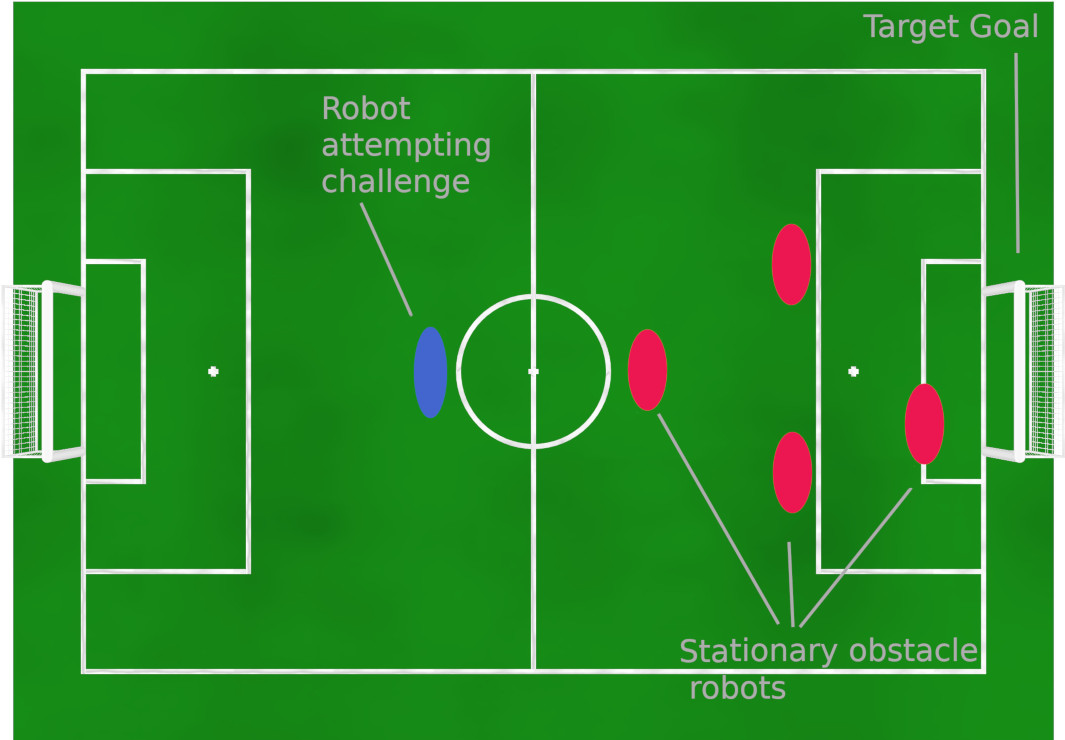
\includegraphics[width=1.0\textwidth]{figs/obstacle_challenge_2021.jpeg}
	\caption{Challenge overview (positions, sizes and distances are not exact)}
\end{figure}

The challenged robot may wear any jersey legal in RoboCup SPL competition or no jersey at all (as decided by the participating team). The jerseys of the obstacle robots will be given as part of the challenge and are either the home or away colour of the participating team or no jersey at all.

The participating team is free to choose which of their goals is used as a target.

The order the obstacles are set up in (i.e., which kind of obstacle is placed in which position, the offset side of the one stationary robot) and their jersey colours are randomized by dice throw (or similar randomization tool) during the competition. The participating team will be told the exact setup of the obstacle robots while setting up the challenge. The judge will give the exact setup of the obstacles and will verify the correct field setup. Thus, no team is aware of the exact setup beforehand. Due to this randomization teams might be challenged with any of the setups given in the examples of figure \ref{fig:possible_obstacle_setups}.

\begin{figure}[ht]
    \centering
	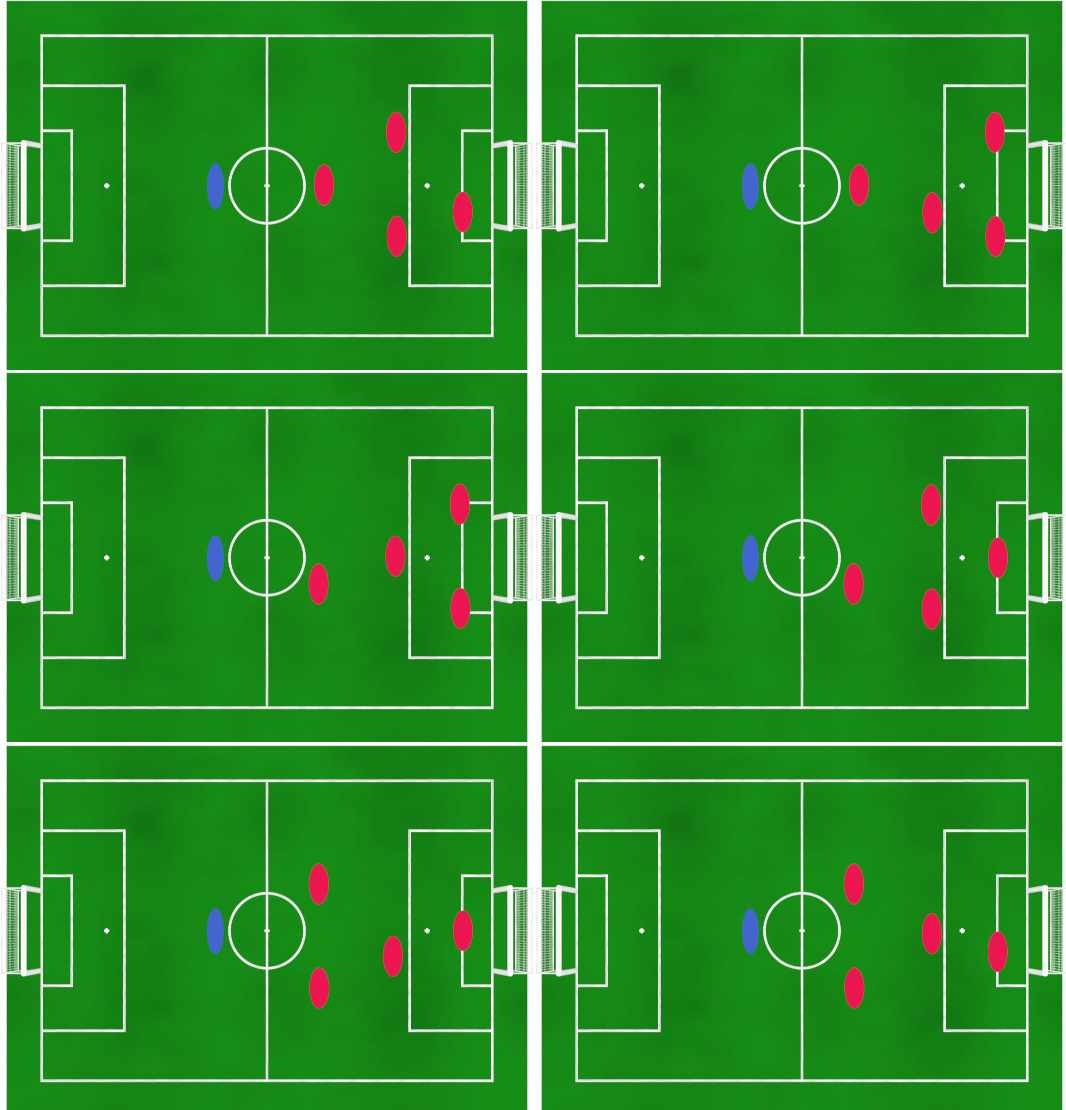
\includegraphics[width=0.8\textwidth]{figs/obstacle_challenge_2021_a.jpeg}
	\caption{Possible obstacle setups encountered during the challenge (not an exhaustive list of all possible cases)}
	\label{fig:possible_obstacle_setups}
\end{figure}

\subsection{Scoring}

The challenged robot is tasked to advance with the ball into the target goal. Both dribbling and kicks are permitted to move the ball. The maximum distance for goal shots is restricted for this challenge. Shots that do not score a goal are unrestricted.

Shots into the goal are only allowed with the centre of the ball being within 1.3 meter from the end field line. This threshold is at the same height as the penalty cross (see dimension I in figure \ref{fig:field_dim}).

Goals shot from a larger distance do not complete the challenge. In this case, the ball is moved back to the starting position by the local challenge assistant and the robot must score another goal according to the rules of the challenge.

Teams are scored by the time it took to move the ball into the goal (rounded up to full seconds). Lower durations are better. Teams are required to score three goals during this challenge. The obstacle setup will be randomized for each of the three runs to score a goal. The final score used is the median of all three runs to score a goal. 

In case of two or more teams being tied on a final score: tied teams are required to repeat the challenge and score two more goals. The final score is recalculated to be the median of all five runs to score a goal. Ties after five runs to score a goal are decided by coinflip.

If the ball is moved out of the field a local challenge assistant takes the ball and places it on the kick-off point.

Touching an obstacle with the ball increases the scored duration of the current run on the goal by five seconds. Touching an obstacle with the challenged robot increases the scored duration of the current run on the goal by 10 seconds.

A robot has at most five minutes (penalties excluded) to complete on run to score a goal.

The team with the lowest final score time is the winner of the challenge. The team with the second lowest time is awarded second place in this challenge (and so on \ldots).

\subsection{Challenge management and planning}

The date and time for the challenge will be announced as part of RoboCup 2021 communication. At least 15 minutes leading up to the challenge the participating teams are given the exact setup of obstacles as determined by randomization.

Participating teams must be ready to compete in the challenge within 15 minutes of being given the obstacle setup. At the end of setup time the challenged robot must be able to stand still and upright (head movement is allowed) and await the start of the challenge. The participating team may use up to 10 minutes to update the challenge setup in-between runs to score a goal. Charging robots is allowed in-between runs. Changing the software used for this challenge is not allowed between runs.

Participating teams must start the robot behaviour of their competing robot via a single chest button press. (This mimics the chest button behaviour of switching between playing and penalized state from previous SPL competitions, \cf Figure~\ref{fig:robot_states}) The participating robot must navigate autonomously and cannot be remote controlled during the challenge.

As part of the challenge the participating team must stream their robot navigating the field (\cf Section \ref{sec:streaming_setup}). Details will be scheduled as part of RoboCup 2021 communication.

\subsection{Non-standard fields}

Teams may compete in this challenge on fields smaller than the standard SPL field, given that:

\begin{itemize}
	\item the area of the artificial turf is big enough to set up the challenge. At least 6 meters long and 4 meters wide.
	\item the distance in-between the goalposts is the same as a standard SPL goal construction (\cf figure \ref{fig:goal_dimensions}).
\end{itemize}

Teams are not required to move field lines for this challenge.

During setup of this challenge all measurements and distances must be used as if the challenge is set up on a standard SPL field.

Example: Assuming a team is setting up on a smaller field where the distance from goal to goal is 75\% of a standard SPL field. The ball is not placed in the centre circle as marked by field lines as the ball would be closer to the target goal compared to a standard SPL field. Instead, the ball is placed independent of centre circle markings so the distance between ball and goal is the same as standard SPL field. All other placements follow the same principle.
